\documentclass{standalone}
\usepackage{tikz}
%\usetikzlibrary{patterns}
\begin{document}
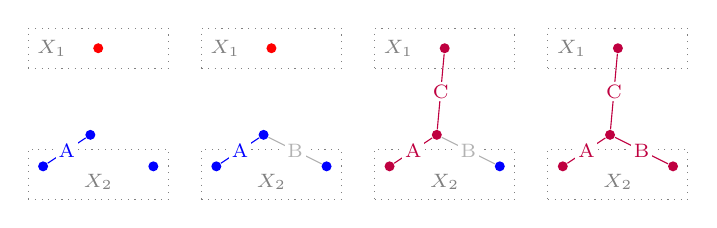
\begin{tikzpicture}

%\fill[fill=none] (-1,0) rectangle (7.6,-1);

\begin{scope}[shift={(0,0)}]
\node[rectangle,draw,dotted,color=black!50,
   inner sep=0,minimum height=0.2in,minimum width=0.7in] (x1) at (0,0) {};
\node[right,color=black!50] at (x1.west) {\scriptsize $X_1$};
\node[rectangle,draw,dotted,color=black!50,
   inner sep=0,minimum height=0.25in,minimum width=0.7in] (x2) at (0,-1.6) {};
\node[above,color=black!50] at (x2.south) {\scriptsize $X_2$};
\node[circle,inner sep=0,minimum size=0.05in,fill=red] (c) at (0,0) {};
\node[circle,inner sep=0,minimum size=0.05in,fill=blue] (a) at (-0.7,-1.5) {};
\node[circle,inner sep=0,minimum size=0.05in,fill=blue] (b) at ( 0.7,-1.5) {};
\node[circle,inner sep=0,minimum size=0.05in,fill=blue] (n) at (-0.1,-1.1) {};
\draw[blue] (a) -- (n) node[pos=.5,fill=white,inner sep=1] {\scriptsize A};
%\draw[black] (b) -- (n) node[pos=.5,fill=white,inner sep=1] {\scriptsize B};
%\draw[black] (c) -- (n) node[pos=.5,fill=white,inner sep=1] {\scriptsize C};
\end{scope}

\begin{scope}[shift={(2.2,0)}]
\node[rectangle,draw,dotted,color=black!50,
   inner sep=0,minimum height=0.2in,minimum width=0.7in] (x1) at (0,0) {};
\node[right,color=black!50] at (x1.west) {\scriptsize $X_1$};
\node[rectangle,draw,dotted,color=black!50,
   inner sep=0,minimum height=0.25in,minimum width=0.7in] (x2) at (0,-1.6) {};
\node[above,color=black!50] at (x2.south) {\scriptsize $X_2$};
\node[circle,inner sep=0,minimum size=0.05in,fill=red] (c) at (0,0) {};
\node[circle,inner sep=0,minimum size=0.05in,fill=blue] (a) at (-0.7,-1.5) {};
\node[circle,inner sep=0,minimum size=0.05in,fill=blue] (b) at ( 0.7,-1.5) {};
\node[circle,inner sep=0,minimum size=0.05in,fill=blue] (n) at (-0.1,-1.1) {};
\draw[blue] (a) -- (n) node[pos=.5,fill=white,inner sep=1] {\scriptsize A};
\draw[black!30] (b) -- (n) node[pos=.5,fill=white,inner sep=1] {\scriptsize B};
%\draw[black] (c) -- (n) node[pos=.5,fill=white,inner sep=1] {\scriptsize C};
\end{scope}

\begin{scope}[shift={(4.4,0)}]
\node[rectangle,draw,dotted,color=black!50,
   inner sep=0,minimum height=0.2in,minimum width=0.7in] (x1) at (0,0) {};
\node[right,color=black!50] at (x1.west) {\scriptsize $X_1$};
\node[rectangle,draw,dotted,color=black!50,
   inner sep=0,minimum height=0.25in,minimum width=0.7in] (x2) at (0,-1.6) {};
\node[above,color=black!50] at (x2.south) {\scriptsize $X_2$};
\node[circle,inner sep=0,minimum size=0.05in,fill=purple] (c) at (0,0) {};
\node[circle,inner sep=0,minimum size=0.05in,fill=purple] (a) at (-0.7,-1.5) {};
\node[circle,inner sep=0,minimum size=0.05in,fill=blue] (b) at ( 0.7,-1.5) {};
\node[circle,inner sep=0,minimum size=0.05in,fill=purple] (n) at (-0.1,-1.1) {};
\draw[purple] (a) -- (n) node[pos=.5,fill=white,inner sep=1] {\scriptsize A};
\draw[black!30] (b) -- (n) node[pos=.5,fill=white,inner sep=1] {\scriptsize B};
\draw[purple] (c) -- (n) node[pos=.5,fill=white,inner sep=1] {\scriptsize C};
\end{scope}

\begin{scope}[shift={(6.6,0)}]
\node[rectangle,draw,dotted,color=black!50,
   inner sep=0,minimum height=0.2in,minimum width=0.7in] (x1) at (0,0) {};
\node[right,color=black!50] at (x1.west) {\scriptsize $X_1$};
\node[rectangle,draw,dotted,color=black!50,
   inner sep=0,minimum height=0.25in,minimum width=0.7in] (x2) at (0,-1.6) {};
\node[above,color=black!50] at (x2.south) {\scriptsize $X_2$};
\node[circle,inner sep=0,minimum size=0.05in,fill=purple] (c) at (0,0) {};
\node[circle,inner sep=0,minimum size=0.05in,fill=purple] (a) at (-0.7,-1.5) {};
\node[circle,inner sep=0,minimum size=0.05in,fill=purple] (b) at ( 0.7,-1.5) {};
\node[circle,inner sep=0,minimum size=0.05in,fill=purple] (n) at (-0.1,-1.1) {};
\draw[purple] (a) -- (n) node[pos=.5,fill=white,inner sep=1] {\scriptsize A};
\draw[purple] (b) -- (n) node[pos=.5,fill=white,inner sep=1] {\scriptsize B};
\draw[purple] (c) -- (n) node[pos=.5,fill=white,inner sep=1] {\scriptsize C};
\end{scope}

\end{tikzpicture}%
\end{document}
